\scanpage{36}
\mspage{3}

a) \(K^\sigma=K\) --- on trouve ess.\textsuperscript{t} les points réels de
\(M_{0,\unsure{5|\bar I}}^{!}\simeq\mathrm{Sym}_2^*(U_{0,3})\),
\deleted{\unsure{Le cas|un cas}} de dim réelle \(2\) : contient le cas \(1^\circ\) (pentagonal)

b) \(\operatorname{Card}K^\sigma=3\), En prenant un repère \(0,1,\infty\) dans \(K^\sigma\), on trouve que
\[
K=\{0,1,\infty,\lambda,\bar\lambda\},\quad
\lambda\in\text{demi-plan de Poincaré},\quad\text{dim réelle }2.
\]
Contient le cas \(3^\circ\) (bitétraédral)
\margin{OPS \(\sigma z=\bar z\) \deleted{\unsure{pour} \(\sigma z=\bar z\)}}

c) \(\operatorname{Card}K^\sigma=1\), i.e. \deleted{\unsure{?}} \(K^\sigma=\{P\}\),
\inserted{\unsure{Soit} \(K\setminus K^\sigma=I\), donc}
\deleted{On \unsure{prend comme repère|prend pour coordonnées|peut prendre comme points} \(\unsure{t_0|\infty}\), et on choisit un p\textsuperscript{t} \(0\) tel que \(0=\sigma0\). \unsure{OP|\(\sigma P\)}}

\((\Sigma,I)\) est un syst. de \(4\) pts sur une sphère complexe,
\deleted{muni d’} \inserted{\unsure{admettant}} un \unsure{antiautomorphisme|anti-isomorphisme}
\deleted{\(\unsure{\sigma}\)} involutif (``conjugaison''), ils sont bien connus et de dim
modulaire \uline{réelle} \(1\), de plus le choix d’un p\textsuperscript{t}
réel supplémentaire \(P\) fait une dim. de
plus, soit dim réelle totale \(2\) encore.
(Contient le cas pyramidal carré, \(2^\circ\))

\figure{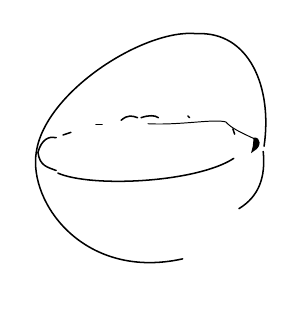
\begin{tikzpicture}[x=.011cm,y=-.011cm,line width=.55pt,line cap=round,line join=round]
\draw (289,1180) .. controls (176,1205) and (111,1116) .. (120,1057)
 .. controls (130,987) and (245,914) .. (305,920)
 .. controls (366,917) and (393,982) .. (383,1050);
\draw (382,1056) .. controls (385,1086) and (377,1108) .. (354,1122);
\draw (122,1057) .. controls (126,1042) and (135,1038) .. (143,1040);
\draw (151,1037)--(160,1034);
\draw (189,1025)--(196,1025);
\draw (218,1020) .. controls (226,1013) and (231,1015) .. (237,1017);
\draw (241,1017) .. controls (250,1014) and (257,1014) .. (261,1017);
\draw (295,1015)--(297,1017);
\draw[line width=.35pt] (249,1024) .. controls (286,1026) and (326,1018) .. (339,1022)
 .. controls (345,1029) and (356,1034) .. (371,1041);
\draw (347,1030)--(349,1036);
\draw (122,1057) .. controls (124,1073) and (133,1074) .. (143,1078);
\draw (145,1081) .. controls (184,1098) and (305,1092) .. (348,1064);
\fill (371,1040) .. controls (380,1039) and (380,1051) .. (372,1055)
 --(368,1058)--(370,1050)--cycle;
\end{tikzpicture}}

\figure{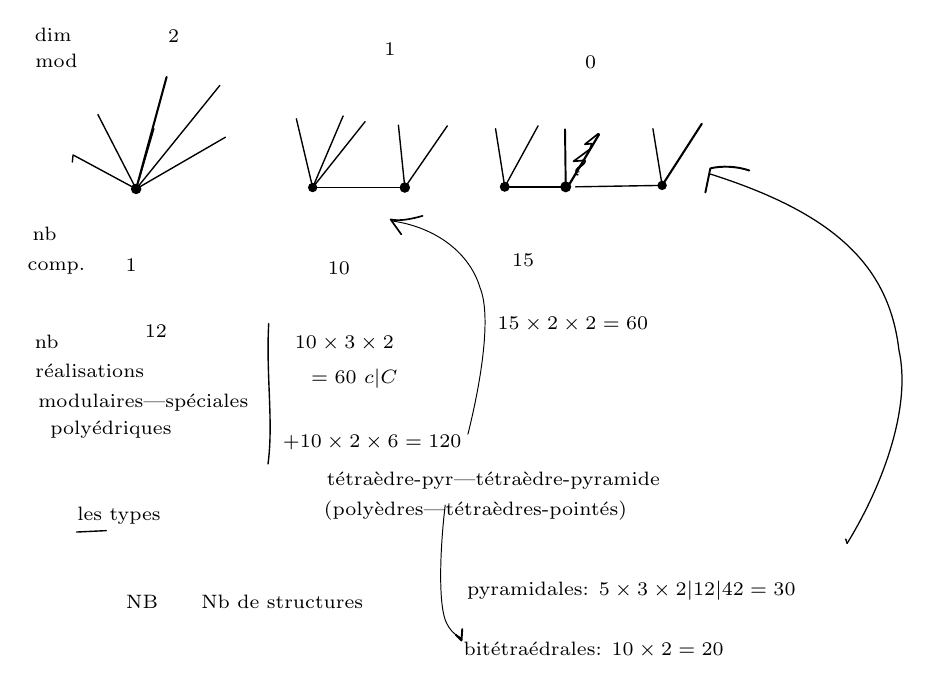
\begin{tikzpicture}[x=.009cm,y=-.009cm,line width=.5pt,line cap=round,line join=round,font=\scriptsize,inner sep=0pt]
\node[anchor=west] at (30,1535) {dim};
\node[anchor=west] at (31,1572) {mod};
\node at (227,1538) {$2$};
\node at (532,1556) {$1$};
\node at (815,1575) {$0$};
% Five free branches at a single vertex.
\draw (174,1753)--(85,1705)--(84,1715);
\draw (174,1753)--(120,1648);
\draw[line width=.75pt] (174,1753)--(217,1595);
\draw (178,1740)--(199,1668);
\draw (174,1753)--(292,1607);
\draw (174,1753)--(300,1680);
\fill (174,1753) circle (1.9pt);
% Two joined vertices and their three plus two branches.
\draw (423,1751)--(553,1751);
\draw (423,1751)--(400,1654);
\draw (423,1751)--(466,1650);
\draw (423,1751)--(497,1658);
\draw (553,1751)--(544,1663);
\draw (553,1751)--(613,1664);
\fill (423,1751) circle (1.7pt);
\fill (553,1751) circle (1.9pt);
% The sloping extra middle branch is crossed out; the upright remains.
\draw (694,1750)--(780,1750);
\draw (794,1750)--(916,1748);
\draw (694,1750)--(681,1668);
\draw (694,1750)--(741,1664);
\draw[line width=.7pt] (780,1750)--(779,1669);
\draw[line width=.8pt] (783,1750)--(827,1676);
\begin{scope}[shift={(760,1645)}]
\draw[line width=.6pt] (37,88) .. controls (32,89) and (33,81) .. (44,74)
 .. controls (50,69) and (47,65) .. (43,68)
 -- (31,69) -- (54,52) -- (57,44) -- (47,45) -- (66,30);
\draw[line width=.35pt] (39,84) .. controls (31,85) and (33,79) .. (43,74);
\end{scope}
\draw (916,1748)--(903,1668);
\draw[line width=.75pt] (916,1748)--(972,1661);
\fill (694,1750) circle (1.8pt);
\fill (780,1750) circle (2pt);
\fill (916,1748) circle (1.7pt);
\node[anchor=west] at (27,1816) {nb};
\node[anchor=west] at (20,1865) {comp.};
\node at (167,1860) {$1$};
\node at (460,1865) {$10$};
\node at (720,1854) {$15$};
\node at (202,1954) {$12$};
\node[anchor=west] at (30,1968) {nb};
\node[anchor=west] at (31,2010) {réalisations};
\node[anchor=west] at (35,2054) {\unsure{modulaires|spéciales}};
\node[anchor=west] at (52,2092) {\deleted{\unsure{polyédriques}}};
\draw (361,1943) .. controls (357,2015) and (368,2082) .. (360,2141);
\node[anchor=west] at (397,1971) {$10\times3\times2$};
\node[anchor=west] at (420,2020) {$=60\ \unsure{c|C}$};
\node[anchor=west] at (380,2110) {$+10\times2\times6=120$};
\node[anchor=west] at (683,1944) {$15\times2\times2=60$};
\node[anchor=west] at (442,2164) {\deleted{\unsure{tétraèdre-pyr|tétraèdre-pyramide}}};
\node[anchor=west] at (438,2207) {\inserted{(\unsure{polyèdres|tétraèdres}-pointés)}};
\node[anchor=west] at (90,2214) {\deleted{\unsure{les types}}};
\draw (90,2237)--(132,2235);
\node[anchor=west] at (159,2335) {\uline{NB}};
\node[anchor=west] at (265,2335) {Nb de structures};
\node[anchor=west] at (640,2320) {pyramidales: $5\times3\times\unsure{2|\deleted{1}\inserted{2}|\deleted{4}\inserted{2}}=30$};
\node[anchor=west] at (635,2404) {bitétraédrales: $10\times2=20$};
% Open upper heads, a hooked right tail, and a separate lower arrow.
\begin{scope}[shift={(525,1695)}]
\draw[line width=.35pt] (117,404) .. controls (137,324) and (150,235) .. (134,197)
 .. controls (120,150) and (74,112) .. (9,103);
\draw[line width=.6pt] (23,122) -- (8,101) .. controls (21,104) and (39,100) .. (53,96);
\draw[line width=.45pt] (652,558) .. controls (703,475) and (743,365) .. (725,285)
 .. controls (711,165) and (632,92) .. (459,37);
\draw[line width=.7pt] (452,63) -- (459,29)
 .. controls (475,25) and (497,26) .. (514,32);
\draw[line width=.5pt] (652,558) -- (650,552);
\draw[line width=.35pt] (85,504) .. controls (78,562) and (75,637) .. (85,666)
 .. controls (91,681) and (99,687) .. (107,691);
\draw[line width=.68pt] (100,687) -- (108,695) -- (109,679);
\end{scope}
\end{tikzpicture}}

\figure{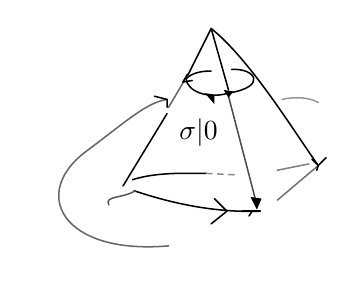
\begin{tikzpicture}[x=.02cm,y=-.02cm,line width=.55pt,line cap=round,line join=round]
\draw (1235,2700)--(1220,2730);
\draw[black!60] (1218,2733)--(1208,2750);
\draw (1207,2754)--(1179,2800);
\draw (1235,2700) .. controls (1260,2720) and (1288,2766) .. (1303,2787);
\draw (1235,2700)--(1246,2739);
\draw[black!70] (1246,2743)--(1264,2812);
\fill (1260,2807)--(1264,2815)--(1267,2808)--cycle;
\draw (1185,2796) .. controls (1201,2791) and (1219,2792) .. (1232,2792);
\draw[black!45,dash pattern=on 2pt off 2pt] (1232,2792)--(1252,2793);
\draw[black!50] (1277,2790)--(1297,2786);
\draw[black!55] (1277,2809)--(1303,2787);
\draw (1303,2787)--(1308,2782);
\draw (1299,2783)--(1303,2787)--(1302,2790);
\draw (1186,2803) .. controls (1210,2811) and (1237,2817) .. (1266,2816);
\draw (1237,2808)--(1245,2816)--(1235,2824);
\draw[line width=.9pt] (1255,2816)--(1266,2816);
\draw (1261,2816)--(1259,2819);
\draw[black!65] (1170,2812) .. controls (1167,2806) and (1179,2808) .. (1187,2803);
% Outer loop, with the visible head at its upper end.
\draw[black!60] (1208,2838) .. controls (1140,2844) and (1119,2804) .. (1157,2777)
 .. controls (1181,2759) and (1194,2747) .. (1207,2745);
\draw (1199,2743)--(1207,2745)--(1207,2750);
\draw[black!40] (1280,2745) .. controls (1289,2743) and (1298,2744) .. (1303,2747);
% Small upper circuit, its breaks and dark directional contacts.
\draw (1219,2732) .. controls (1223,2728) and (1229,2727) .. (1235,2727);
\draw (1248,2726) .. controls (1263,2725) and (1271,2737) .. (1246,2741)
 .. controls (1233,2745) and (1220,2740) .. (1219,2732);
\draw (1220,2729)--(1217,2734)--(1223,2733);
\fill (1231,2741)--(1237,2748)--(1237,2742)--cycle;
\fill (1243,2739)--(1246,2744)--(1249,2740)--cycle;
\node at (1227,2766) {$\unsure{\sigma|0}$};
\end{tikzpicture}}

\margin{35}
